\documentclass[10pt]{article}
\usepackage[utf8]{inputenc}
\usepackage[activeacute,spanish]{babel}
\usepackage[left=1.5cm,top=1.5cm,right=1.5cm, bottom=1.5cm,letterpaper, includeheadfoot]{geometry}

\usepackage{amssymb, amsmath, amsthm}
\usepackage{graphicx}
\usepackage{hyperref}
\usepackage{lmodern,url}
\usepackage{paralist} %util para listas compactas
\usepackage{xcolor}
\usepackage{bbm}
\usepackage{mathrsfs}
\usepackage{bbm}

%========PAQUETES AGREGADOS===========
%Pseudocodigo
\usepackage{pseudocode}
\usepackage[portuguese, boxruled]{algorithm2e}
\usepackage{wrapfig}
\usepackage{multicol}
\usepackage{graphicx}
\usepackage{caption}
\usepackage{subcaption}
%\captionsetup[table]{labelformat=empty}
\captionsetup[subfigure]{labelformat=empty}
\usepackage{cancel}
%====================================

\usepackage{fancyhdr}
\pagestyle{fancy}
\fancypagestyle{plain}{%
\fancyhf{}
\lhead{\footnotesize\itshape\bfseries\rightmark}
\rhead{\footnotesize\itshape\bfseries\leftmark}
}


% macros
\newcommand{\Q}{\mathbb Q}
\newcommand{\R}{\mathbb R}
\newcommand{\N}{\mathbb N}
\newcommand{\Z}{\mathbb Z}
\newcommand{\C}{\mathbb C}
\newcommand{\BigO}{\mathcal{O}}
%Teoremas, Lemas, etc.
\theoremstyle{plain}
\newtheorem{teo}{Teorema}
\newtheorem{lem}{Lema}
\newtheorem{prop}{Proposición}
\newtheorem{cor}{Corolario}
\newtheorem{obs}{Observación}
\newtheorem{ej}{Ejemplo}
\renewcommand{\qedsymbol}{\rule{0.7em}{0.7em}}
\renewenvironment{proof}{{\bfseries \noindent Demostración}}{ \qed \\}


\theoremstyle{definition}
\newtheorem{defi}{Definición}
% fin macros


\newcommand{\catnum}{7} %numero de catedra
\newcommand{\fecha}{13 de Septiembre 2016 }

%%%%%%%%%%%%%%%%%%

%Macros para este documento
\newcommand{\cin}{\operatorname{cint}}



\begin{document}
%Encabezado
\fancyhead[L]{Facultad de Ciencias Físicas y Matemáticas}
\fancyhead[R]{Universidad de Chile}
\vspace*{-1.2 cm}
\begin{minipage}{0.6\textwidth}
\begin{flushleft}
\hspace*{-0.5cm}\textbf{MA3402-1 Estadística. Primavera 2016}\\
\hspace*{-0.5cm}\textbf{Profesor:} Raul Gouet\\
\hspace*{-0.5cm}\textbf{Escriba:} Manuel Cáceres\\
\hspace*{-0.5cm}\textbf{Fecha:} \fecha
\end{flushleft}
\end{minipage}
\begin{minipage}{0.36\textwidth}
\begin{flushright}

\includegraphics[scale=0.3]{imagenes/fcfm_dcc}
\end{flushright}
\end{minipage}
\bigskip
%Fin encabezado

\begin{center}
\LARGE\textbf{Clase \catnum}
\end{center}
\section{Conjuntos de Confianza}
Modelo paramétrico de siempre $\mathcal{P}= \{\mathbb{P}_{\theta}\colon \theta \in \Theta\} \subseteq \mathbb{R}^k$ y $X$ la observación. En estimación puntual de $g(\theta)$ buscamos $\hat{g}$ tal que $\hat{g}(X)$ se parezca a $g(\theta)$ (uniformemente).\\
La estimación de $g(\theta)$ por conjunto de confianza consiste en buscar o construir un conjunto $S(X)$ (aleatorio) que depende de $X$ tal que contenga a $g(\theta)$ con un ``alto nivel de confianza''.\\
Si $g(\theta) \in \mathbb{R}$ es lógico tomar $S(X)$ como intervalo $S(X) = [L(X),R(X)]$.\\
Si $g(\theta) \in \mathbb{R}^2$, se consideran elipses o rectángulos de confianza.
\begin{defi}
En el esquema clásico de la inferencia paramétrica, un conjunto de confianza $S(X)$ para $g(\theta)$, con nivel $1-\alpha$ satisface:
\begin{align*}
\mathbb{P}_{\theta}(g(\theta) \in S(X)) \ge 1-\alpha,\ \forall \theta \in \Theta, \alpha \in [0,1]
\end{align*}
típicamente $\alpha$ pequeño.\\
\end{defi}
Vamos a resolver parcialmente el problema de intervalos de confianza, es decir, $g(\theta)$ con valores en $\mathbb{R}$.\\
Para motivar utilizamos un caso muy importante, una MAS $X_{1}, X_{2}, \ldots, X_{n}$ del modelo gaussiano $N(\mu, \sigma^2)$ donde supondremos que $\sigma>0$ es conocido. QUeremos construir un intervalo de confianza par $\mu$, haremos estimación intervalar para $\mu$.\\
Para comenzar notemos que $\bar{X} = \frac{1}{n}\sum_{i=1}^n X_{i} \sim N\left(\mu,\frac{\sigma^2}{n}\right)$.\\
Por lo tanto, $Z = \frac{\bar{X}-\mu}{\frac{\sigma}{\sqrt{n}}} = \sqrt{n}\left(\frac{\bar{X}-\mu}{\sigma}\right) \sim N(0,1)$.\\

Buscamos ahora dos valores $z_{\alpha_{1}}, z_{\alpha_{2}}$ tales que
\begin{align*}
\mathbb{P}_{\mu}[z_{\alpha_{1}}\le Z \le z_{\alpha_{2}}] = \int_{z_{\alpha_{1}}}^{z_{\alpha_{2}}}{\phi (t)dt} \ge 1-\alpha
\end{align*}

Para $\alpha \in [0,1]$ ¿Existen $z_{\alpha_{1}} \le z_{\alpha_{2}}$?.\\

Si $\alpha = 0$, entonces $z_{\alpha_{1}}=-\infty$ y $z_{\alpha_{2}}=\infty$, no es una solución válida.\\

Al revés si $\alpha=1$, entonces basta $z_{\alpha_{1}} = z_{\alpha_{2}}$.\\

En una situación intermedia, $\alpha = (0,1)$ tenemos:
\begin{center}
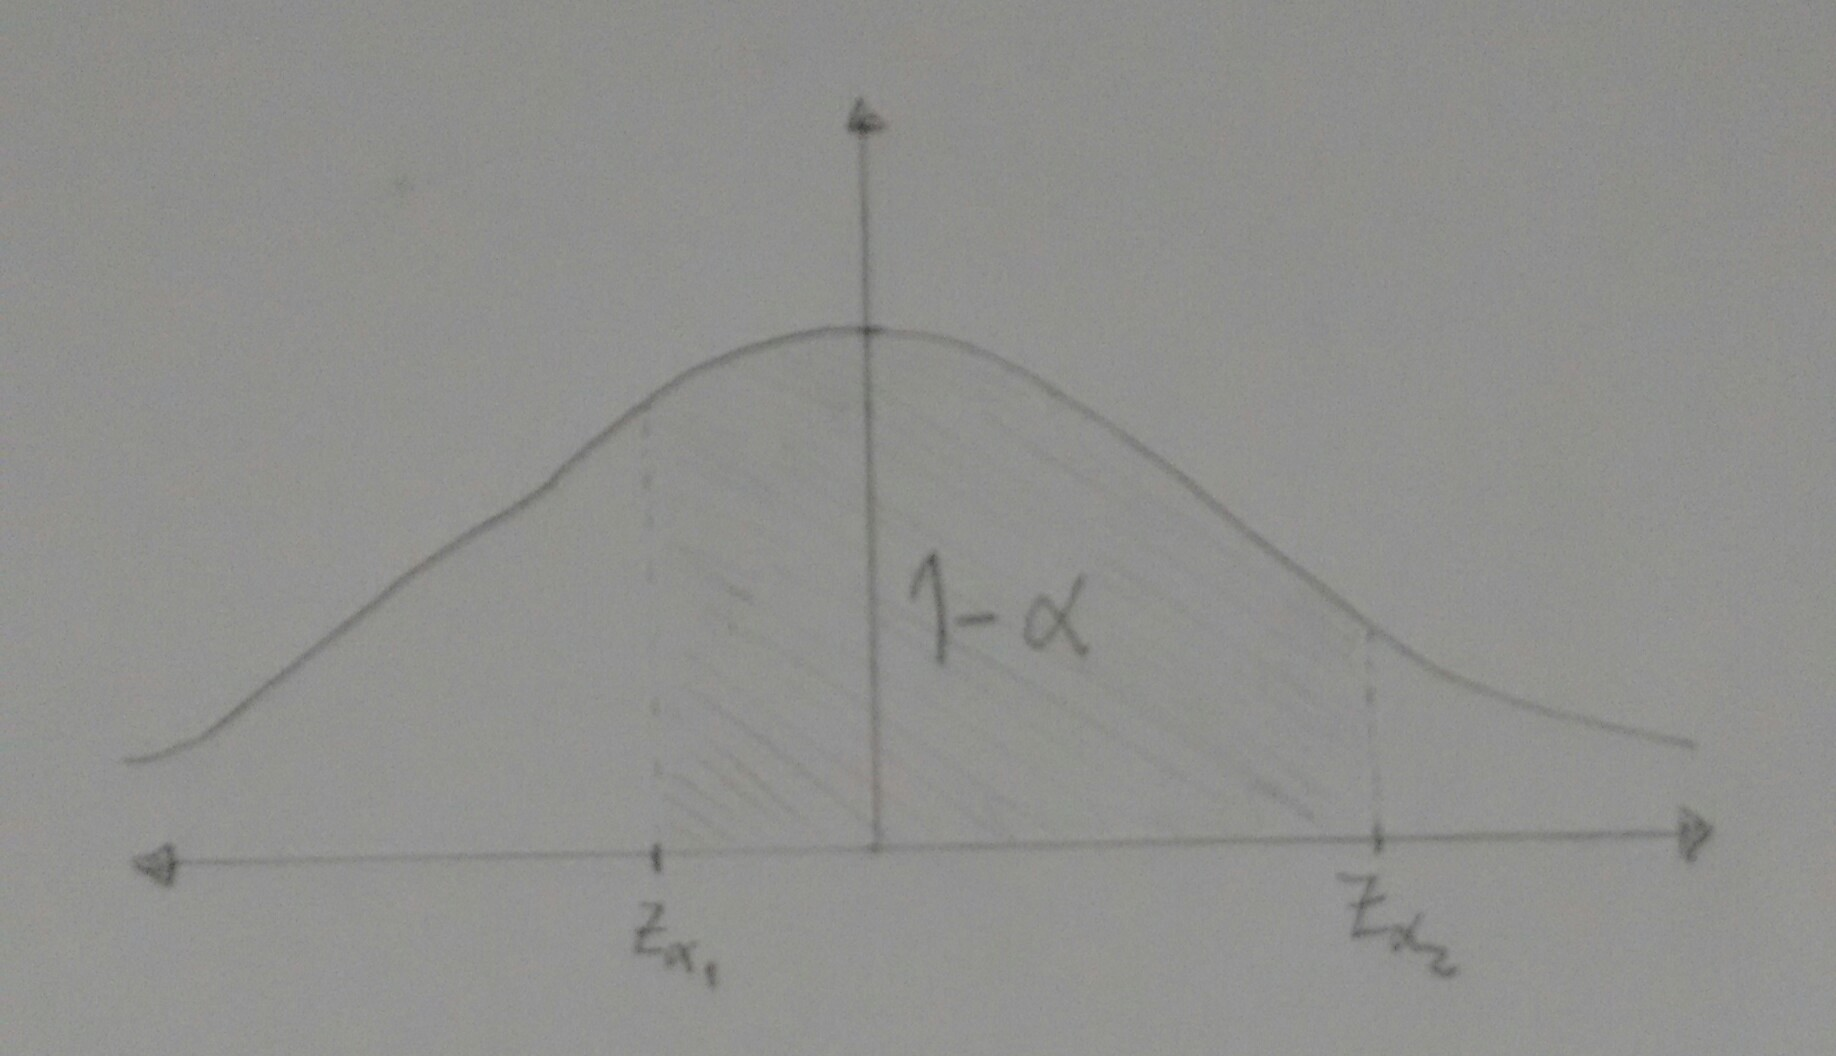
\includegraphics[scale=0.2]{imagenes/normal1.jpg}
\end{center}
Si existen $z_{\alpha_{1}}, z_{\alpha_{2}}$, entonces existen infinitos pues basta mover $z_{\alpha_{1}}$ a la izquierda o $z_{\alpha_{2}}$ a la derecha manteniéndose la desigualdad.\\

La función $t \mapsto \Phi(t)$ es continua, creciente por lo que la ecuación $\Phi(t) = \alpha$ tiene única solución dada por $\Phi^{-1}(\alpha)$
\begin{center}
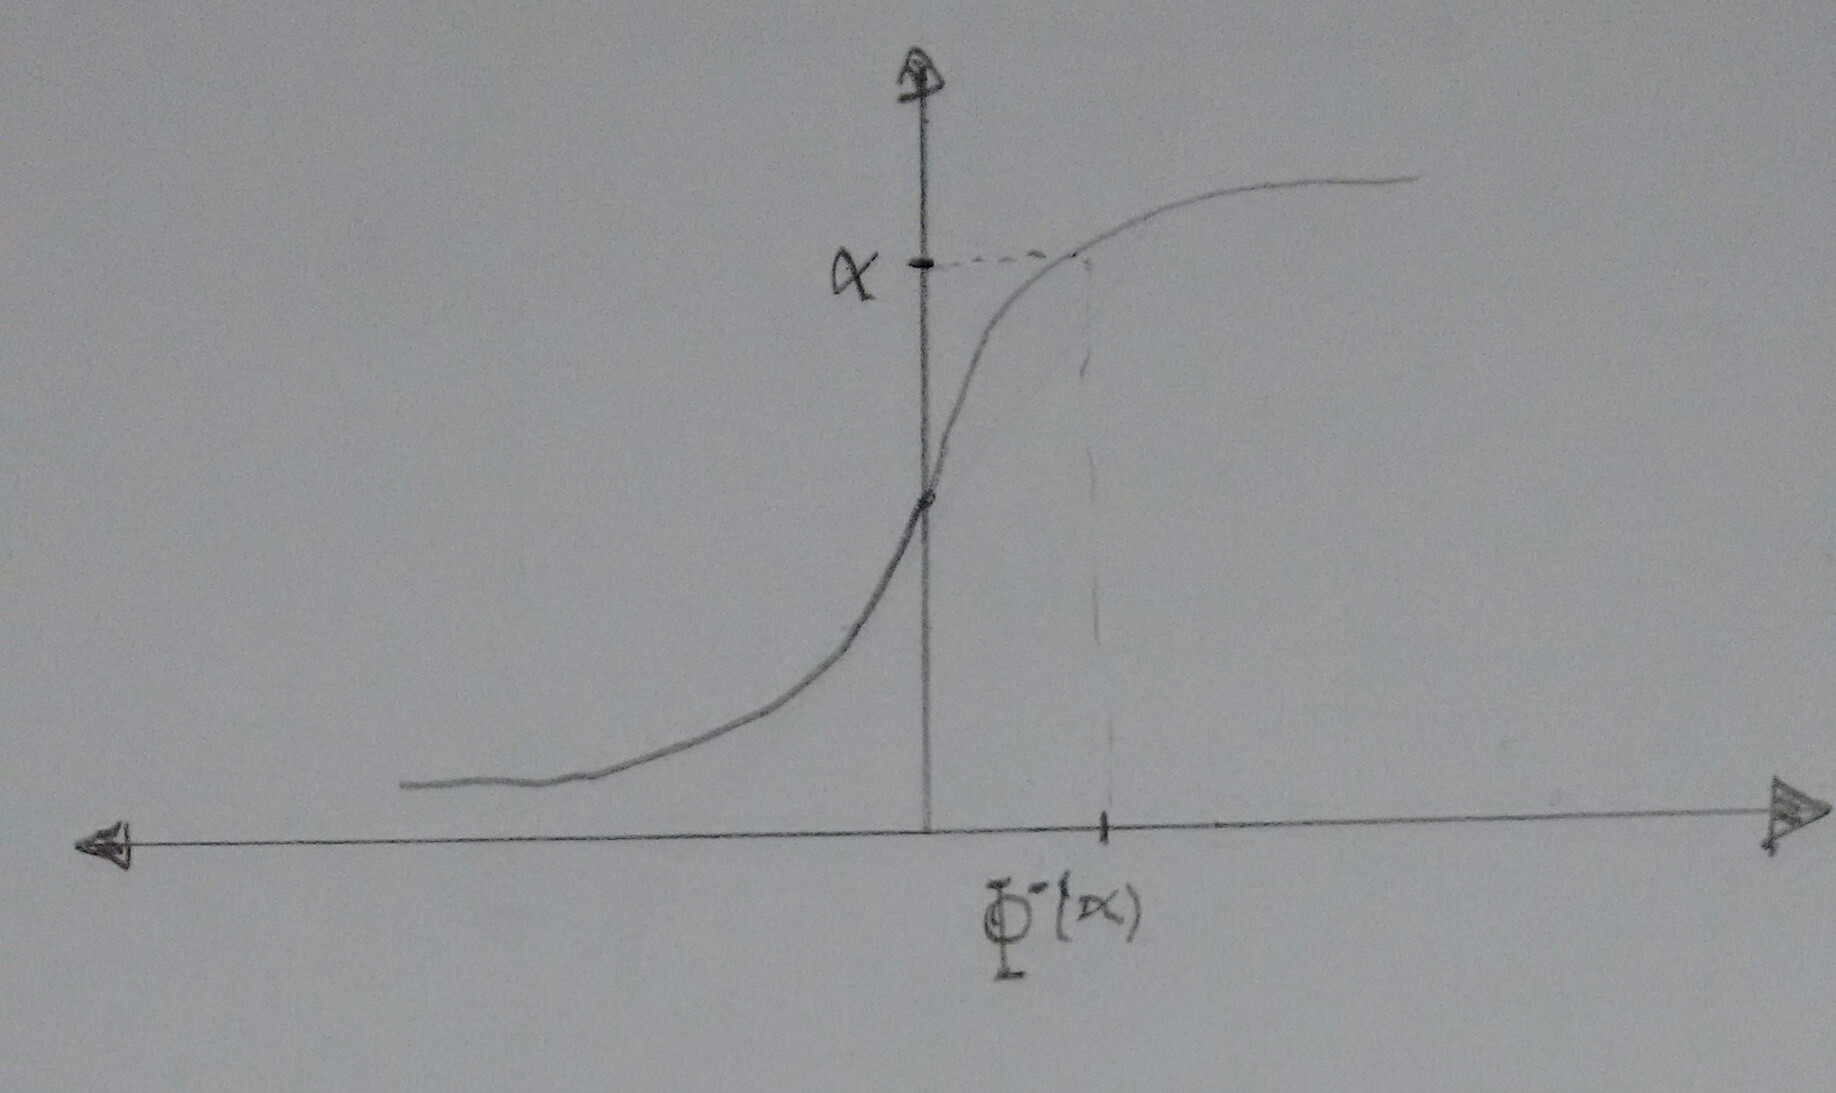
\includegraphics[scale=0.2]{imagenes/normal2.jpg}
\end{center}
Consideremos $\alpha_{1}$ y $\alpha_{2}$ tales que $\alpha_{1}+\alpha_{2}=\alpha$ y definamos $z_{\alpha_{1}} = \Phi^{-1}(\alpha_{1})$ y $z_{\alpha_{2}} = \Phi^{-1}(1-\alpha_{2})$	
\begin{center}
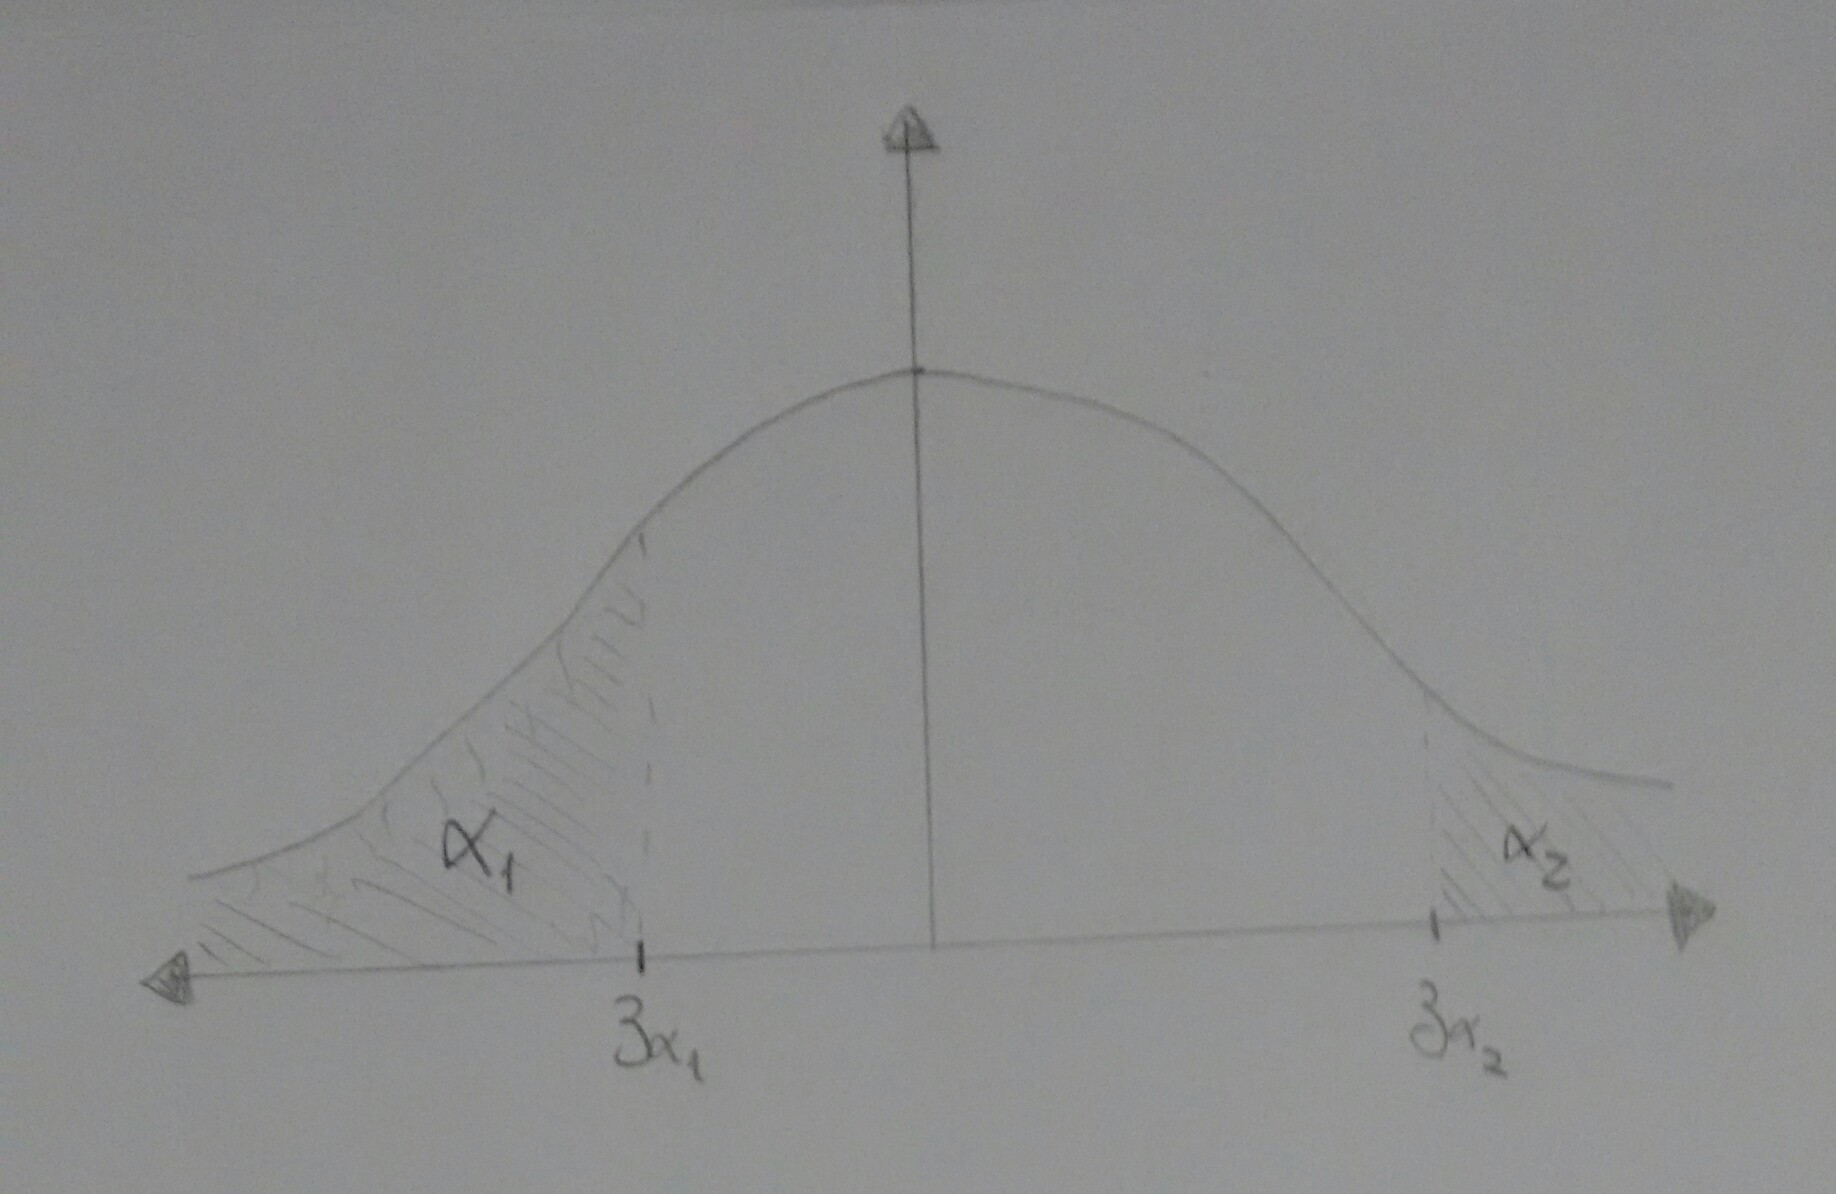
\includegraphics[scale=0.2]{imagenes/normal3.jpg}
\end{center}
Tenemos una solución $z_{\alpha_{1}} < z_{\alpha_{2}}$ asociada (una entre muchas).\\
Ahora trabajamos las desigualdades despejando $\mu$
\begin{align*}
z_{\alpha_{1}} \le \sqrt{n} \frac{\bar{X}-\mu}{\sigma} \le z_{\alpha_{2}} \\
\mathbb{P}_{\mu}(z_{\alpha_{1}} \le Z \le z_{\alpha_{2}}) \le 1 - \alpha, \forall \mu \in \mathbb{R} \\
z_{\alpha_{1}} \frac{\sigma}{\sqrt{n}} \le \bar{X} - \mu \le z_{\alpha_{2}} \frac{\sigma}{\sqrt{n}}\\
\bar{X} - z_{\alpha_{2}} \frac{\sigma}{\sqrt{n}} \le \mu \le \bar{X} - z_{\alpha_{1}} \frac{\sigma}{\sqrt{n}}
\end{align*}
Así
\begin{align*}
\mathbb{P}_{\mu}\left(\mu \in [\bar{X}-z_{\alpha_{2}}\frac{\sigma}{\sqrt{n}}, \bar{X}-z_{\alpha_{1}}\frac{\sigma}{\sqrt{n}}]\right) = 1 - \alpha
\end{align*}
Con lo que tenemos un intervalo de nivel $1-\alpha$ de confianza para $\mu$.\\

Analicemos el intervalo $[\bar{X}-z_{\alpha_{2}}\frac{\sigma}{\sqrt{n}}, \bar{X}-z_{\alpha_{1}}\frac{\sigma}{\sqrt{n}}]$
\begin{enumerate}
\item Si $\sigma$ crece, enconces el largo del intervalo crece (mal pues no queremos intervalos muy largos).
\item Si $n$ crece el intervalo decrece y por ley de los grandes números $\bar{X}\rightarrow \mu$ (lo que es bueno).
\item Si $\alpha_{1}, \alpha_{2}$ decrecen el largo aumenta.
\end{enumerate}
¿Qué valores óptimos podemos escoger para $\alpha_{1}, \alpha_{2}$?\\

Escribimos el problema de optimización:
\begin{align*}
\min_{\alpha_{1}, \alpha_{2}} &z_{\alpha_{1}}-z_{\alpha_{2}}\\
& s.a.\ \alpha_{1}+\alpha_{2}= \alpha
\end{align*}
Que es equivalente a:
\begin{align*}
\min_{\alpha_{1}, \alpha_{2}} &\Phi^{-1}(\alpha_{1})-\Phi^{-1}(\alpha_{2})\\
& s.a.\ \Phi(z_{\alpha_{2}}) - \Phi(z_{\alpha_{2}})= 1-\alpha
\end{align*}
Usando multiplicadores de Lagrange esto conduce a la condición $\phi(z_{\alpha_{1}}) = \phi(z_{\alpha_{2}})$
\begin{center}
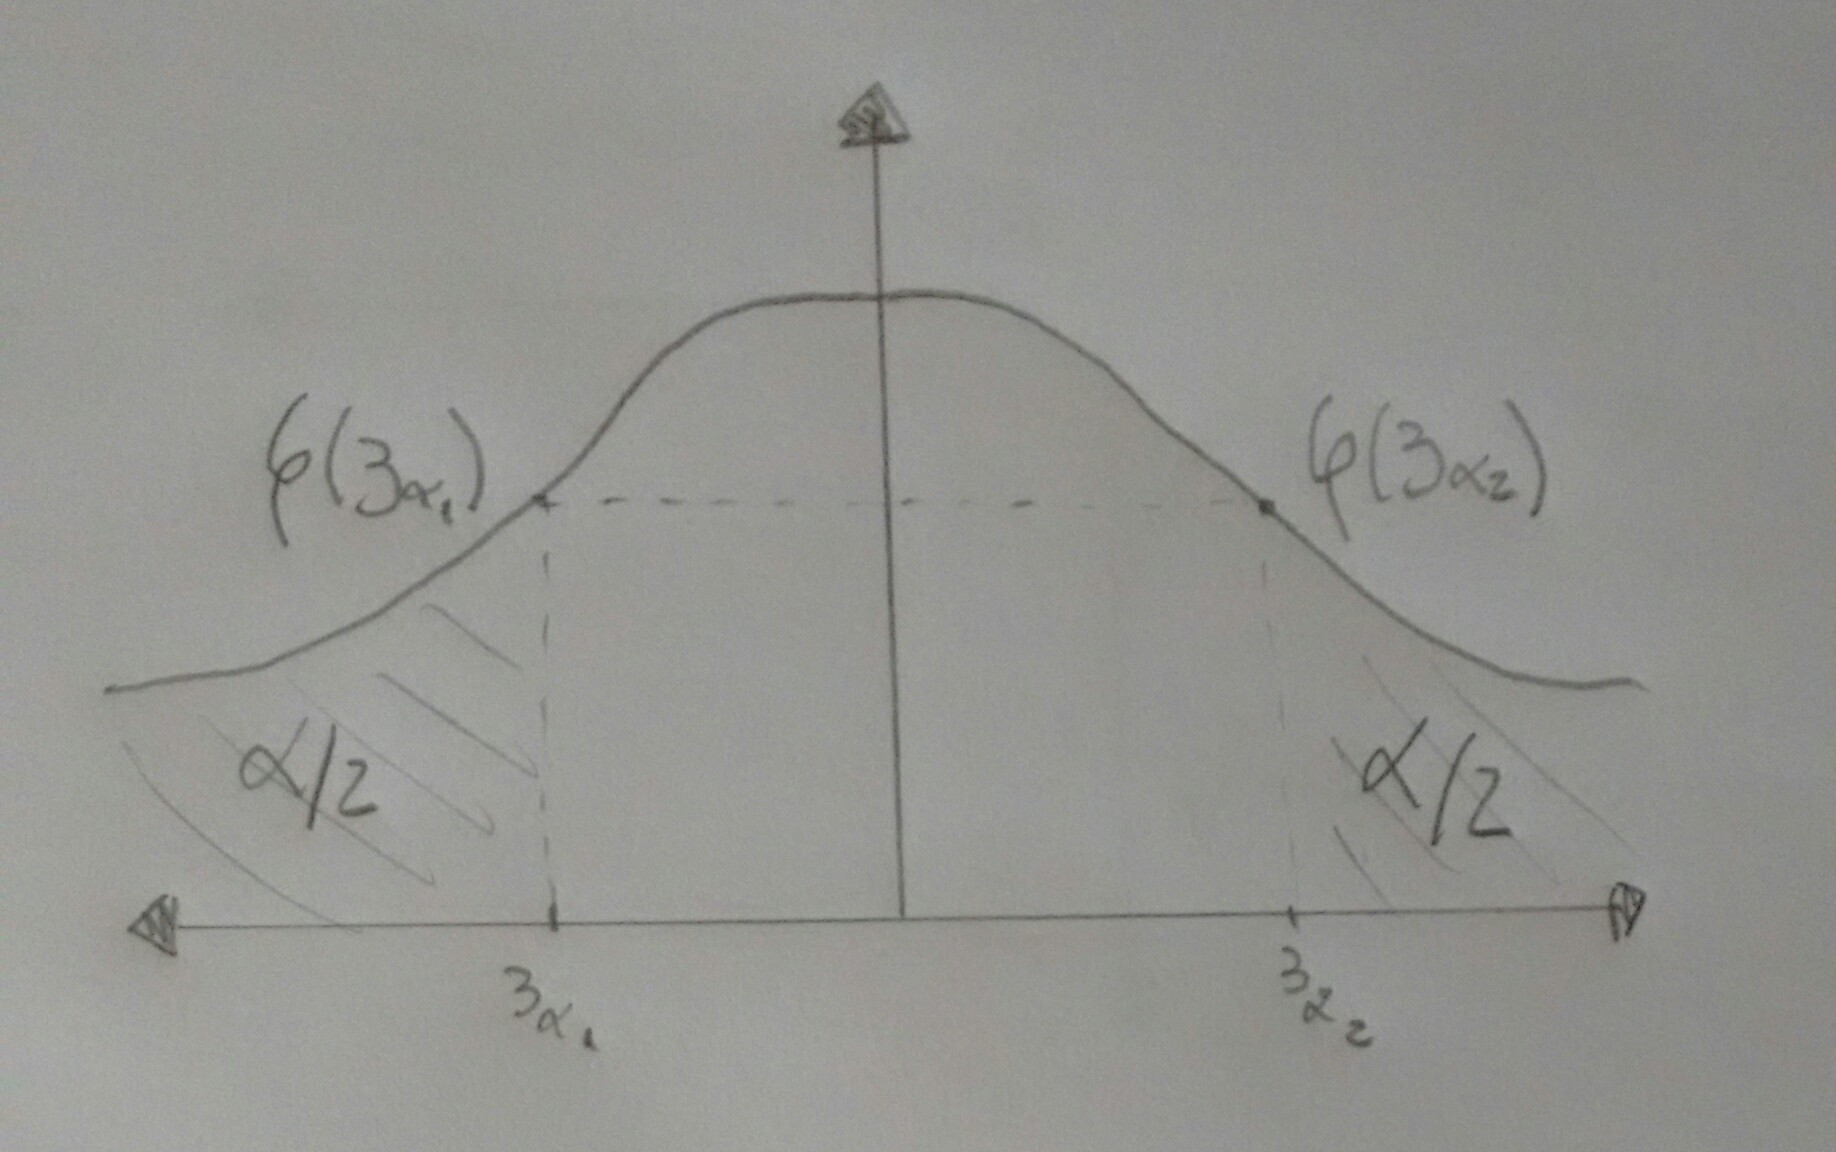
\includegraphics[scale=0.2]{imagenes/normal4.jpg}
\end{center}
Por simetría de $\phi$ resulta $\Phi^{-1}(\alpha/2)= z_{\alpha_{1}} = -z_{\alpha_{2}} = - \Phi^{-1}(1-\alpha/2)$.\\
Definimos $z_{\alpha/2} = \Phi^{-1}(1-\alpha/2)$. Finalmente tenemos el intervalo de nivel $1-\alpha$, más corto posible (basado en esta idea del uso de $Z$), dado por :
\begin{align*}
[\bar{X}-z_{\alpha/2}\frac{\sigma}{\sqrt{n}}, \bar{X}+z_{\alpha/2}\frac{\sigma}{\sqrt{n}}]
\end{align*}
Este es un ejemplo del método llamado ``método del pivote''.\\

El método del pivote para encontrar un intervalo de confianza para una función $g(\theta)$ del parámetro $\theta$ se basa en la existencia de una función $T: \mathfrak{X} \times \Omega \mapsto \mathbb{R}$ medible, tal que $T(x,\omega)$ sea función monótona de $g(\theta), \forall x$ y que la ley de $T(x,\theta)$ no depende de $\theta$, es decir, $\mathbb{P}_{\theta}(T(x,\theta)\le t) = F(t)$, para cierta función de distribución $F$.\\

Teniendo un pivote, buscamos (si existen) $t_{\alpha_{1}}, t_{\alpha_{2}}$ tales que:
\begin{align*}
F(t_{\alpha_{2}})-F(t_{\alpha_{1}}) = \mathbb{P}_{\theta}(t_{\alpha_{1}}\le T(x,\theta)\le t_{\alpha_{2}}) \ge 1-\alpha
\end{align*}
Finalmente, las desigualdades dentro de la probabilidad se resuelven como:
\begin{align*}
g_{1}(X) \le g(\theta) \le g_{2}(X)
\end{align*}
Así $[g_{1}(X),g_{2}(X)]$ es un intervalo de nivel $1-\alpha$ para $g(\theta)$.\\
Ahora hay que encontrar los pivotes.\\

El ejemplo que resolvimos tiene como pivote la función:
\begin{align*}
T(X,\mu) = \frac{\sqrt{n}(\bar{X}-\mu)}{\sigma}
\end{align*}
Veamos otro caso interesante de pivote.\\
Supongamos que queremos un intervalo para $\mu$ basado en $X_{1},X_{2},\ldots,X_{n}$ iid $N(\mu,\sigma^2)$, ambos parámetros desconocidos. $\theta = (\mu,\sigma)$, $g(\theta) = \mu$ y $T(x,\theta)$ sería:
\begin{align*}
T(x,\theta) = \sqrt{n}\frac{\bar{X}-\mu}{\hat{\sigma}}
\end{align*}
Donde $\hat{\sigma} = \hat{\sigma}(X)$ es un estimador puntual desconocido.\\

¿Qué escogemos como estimador?\\
La solución conocida es tomar $\hat{\sigma}^2 = \frac{1}{n-1}\sum_{i=1}^n {(X_{i}-\bar{X})^2}$, pues la ley de $T(x,\theta)$ no depende de $\theta$ y es conocida; se llama ``t de Student, con $(n-1)$ grados de libertad''.
\end{document}
